

%\subsection*{\texttt{center} environment: (standard \LaTeX{})}
\begin{titlepage}
\begin{center}

\Huge
\textbf{به نام خدا}\\[2cm]

\huge
\textbf{گزارش پروژه نهایی }\\[0.5cm]
\textbf{سیستم‌های مخابراتی}\\[1.5cm]

\Large
\textbf{مبین خطیب}\\[0.3cm]
\textbf{99106114}\\[0.5cm]
\end{center}
\end{titlepage}

\newpage
\huge
\section{مقدمه}
\large
در این قسمت دیاگرام فرستنده و گیرنده ترسیم شده که برای حل مسئله از آن استفاده کردیم
\section{پیاده سازی بلوک ها به صورت مجزا}
\large
2.1:
دو تابع Divide و Combine را مطابق خواسته مساله پیاده سازی کردیم. تنها نکته مهم این است که برای نزدیک شدن به حالت Real-Time، درایه های فرد b را در b1 و درایه های زوج را در b2 قرار دادیم. اینگونه میتوان فرض کرد که دو پردازش همزمان و موازی هستند و سرعت ما دوبرابر شده و از طرفی همزمانی نیز رعایت میشود. در تابع Combine نیز همین منطق را در پیش گرفتیم.
\\[0.5cm]
\large
2.2:
تابع PulseShaping را مطابق خواسته سوال طراحی کردیم. به این صورت که به ازای هر بیت 1 در آرایه باینری، یک شکل موج مختص به بیت برابر با 1 و به ازای هر بیت 0 در آرایه باینری، یک شکل موج مختص به بیت برابر با 0 قرار دادیم. ترتیب این ها را نیز رعایت کردیم.
\\[0.5cm]
2.3:
تابع AnalogMod را مطابق خواسته سوال طراحی کردیم. به این صورت که سیگنال ورودی را در توابع سینوس و کسینوس با فرکانس مرکزی ${f}_{c}$ ضرب کردیم و پس از جمع با یکدیگر آن را خروجی دادیم. توابع سینوسی را با فرکانس ${f}_{s}$ نمونه برداری کردیم.
\\[0.5cm]
2.4:
فیلتر هارا به صورت دستی تولید و استفاده کردیم میدانیم که فیلتر حوزه زمان $sinc(t)$ فیلتر پایین گذر در حوزه زمان است. از طرفی طبق قوانین فوریه ای میدانیم $g(t)\leftrightarrow G(f) \Leftrightarrow g(t-{t}_{0})\Leftrightarrow {e}^{-j2{\pi}{f}{t_0}}G(f)  $ بنابر این با ضرب دو نمایی در سیگنال $sinc(t) $میتوانیم فیلتر میانگذر دلخواه را تولید کنیم. با عبور سیگنال ${x}_{transmit}$ از فیلتر ساخته شده سیگنال دریافت شده در دریافت کننده یعنی ${x}_{receive}$ را تولید میکنیم.
\\[0.5cm]
2.5:
کلیت این قسمت مانند تابع AnalogMod میباشد و لازم است که سیگنال را در یک سری سینوس و کسینوس ضرب کنیم و خروجی را تولید کنیم. مشابه همان توضیحات قسمت قبل برای تولید فیلتر پایین گذر از یک تابع $sinc(t) $
تبدیل fft گرفته و سیگنال را از آن عبور میدهیم.
\\[0.5cm]
2.6:
تابع اصلی این تابع است مطابق تعریف میدانیم که Matched Filter برای هرکدام از پالس های ما به صورت روبرو تعریف میشود: $Matched Filter = h(t) = pulse(T-t)$ بنابر این با flip کردن شکل پالس مختص به بیت 1 و 0، MatchedFilter های مربوطه تولید میشوند. پس از آن باید سیگنالی که در ورودی دریافت کرده ایم را با MatchedFilter ها کانوالو کنیم و هر T ثانیه نمونه برداری کنیم. حال برای تصمیم گیری که هر نمونه نشان دهنده بیت 1 بوده یا 0 نیز کافی است که خروجی MatchedFilter متناظر با 1 را با با خروجی متناظر با 0 مقایسه کنیم و هرکدام بزرگتر بود، خروجی همان خواهد بود.
\newpage
\huge
\section{انتقال دنباله تصادفی 0 و 1}
\large
3.1: 
پارامتر های مساله را مطابق خواسته دستور پروژه تنظیم کردیم و موارد اضافه تری را که تنظیم کرده ایم در کد متلب توضیحاتش را کامنت کرده ایم.
\\[1cm]
آ:
\\
خروجی های بلوک را به ترتیب نمایش میدهیم. شکل ها دارای Title، Xlabel و Ylabel میباشند.
\\
\begin{center}
    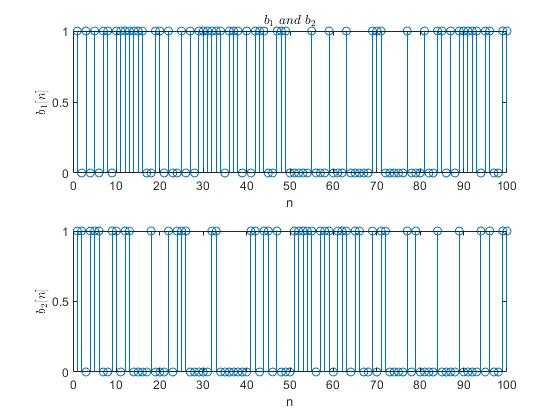
\includegraphics[width=0.9\textwidth]{untitled1.jpg}
\end{center}
\centering
خروجی تابع Divide


newline
\begin{center}
    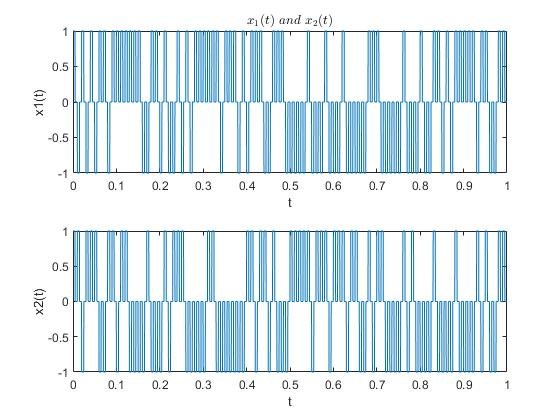
\includegraphics[width=0.9\textwidth]{untitled2.jpg}
\end{center}

\centering
خروجی تابع PulseShaping
 
\begin{center}
    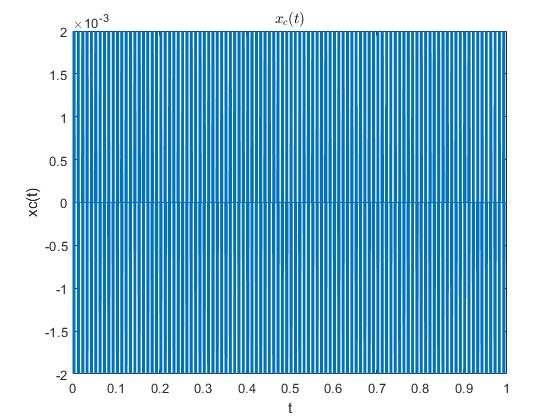
\includegraphics[width=0.9\textwidth]{untitled3.jpg}
\end{center}

\centering
خروجی تابع AnalogMod
 

\begin{center}
    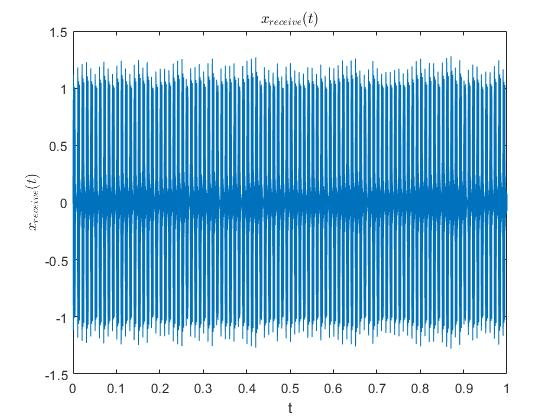
\includegraphics[width=0.9\textwidth]{untitled4.jpg}
\end{center}

\centering
خروجی تابع Channel
 

\begin{center}
    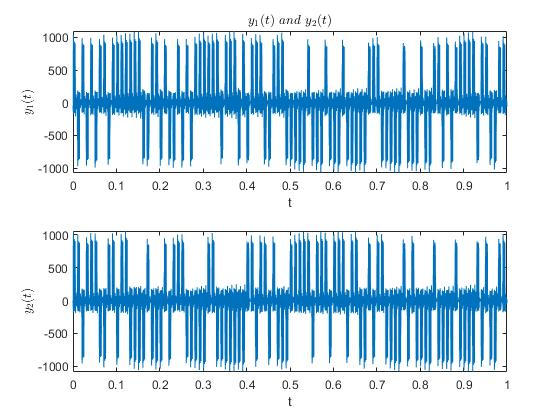
\includegraphics[width=0.9\textwidth]{untitled5.jpg}
\end{center}
\centering
خروجی تابع AnalogDemod
 

\begin{center}
    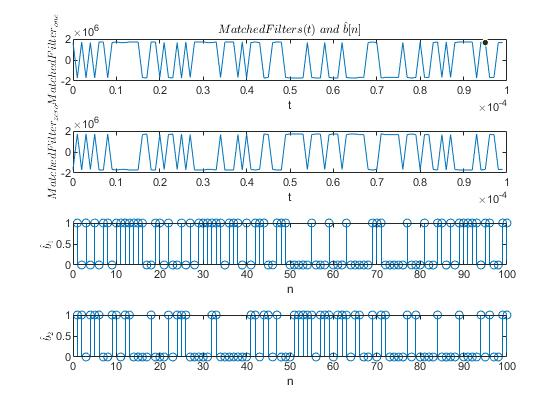
\includegraphics[width=0.9\textwidth]{untitled6.jpg}
\end{center}

\centering
خروجی تابع MatchedFilter
 

\begin{center}
    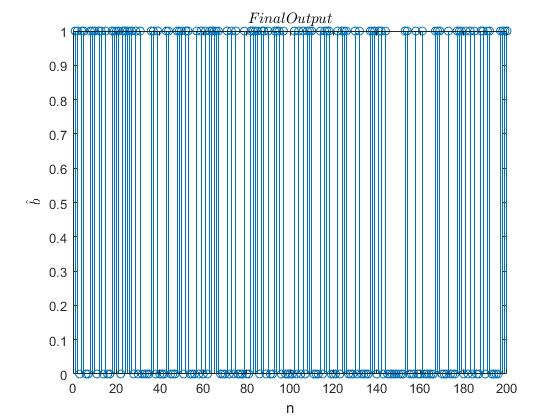
\includegraphics[width=0.9\textwidth]{untitled7.jpg}
\end{center}

\centering
خروجی تابع Combine
 

\begin{center}
    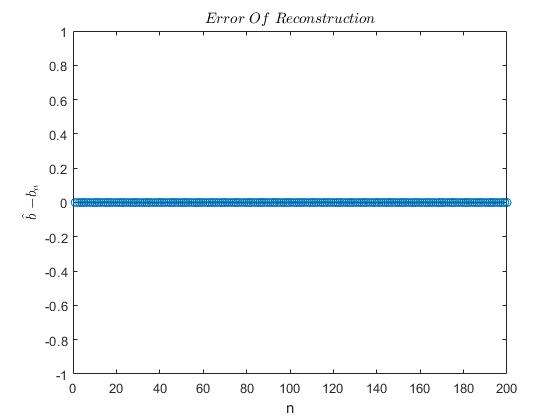
\includegraphics[width=0.9\textwidth]{untitled8.jpg}
\end{center}

\centering
خطای بازسازی


\raggedleft
ب:
\\
با استفاده از دستور normrnd در متلب که متغیر رندوم با توزیع گوسی و میانگین و واریانس دلخواه ما تولید میکند، به سیگنال خروجی از تابع Channel نویز می افزاییم. نتیجه خواسته شده به شرح زیر میباشد:


\begin{center}
    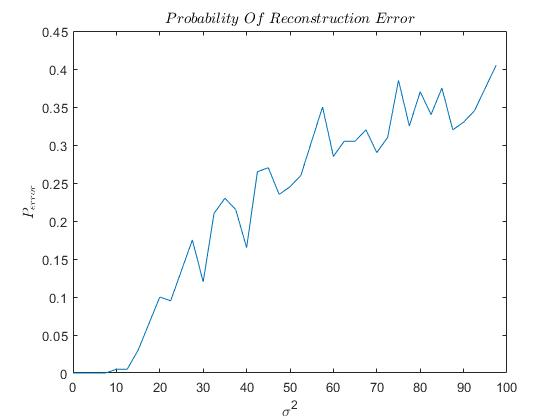
\includegraphics[width=0.9\textwidth]{untitled9.jpg}
\end{center}

\centering
احتمال خطای بازسازی برحسب واریانس نویز کانال
\\[0.5cm]
\raggedleft
\justify
واضح است که این رفتار کاملا مطابق با انتظار ماست. همانطور که در تصویر هم واضح است خطای باز سازی به ازای واریانس های کم نویز صفر است، یعنی دریافت کننده میتواند سیگنالی که آلوده به نویز کوچکی است را با دقت 100 درصد بازسازی کند. اما رفته رفته با افزایش شدت نویز و افزایش واریانس آن، خطای بازسازی افزایش میابد و مطابق انتظارمان،، وقتی که واریانس نویز بیشتر و بیشتر میشود خطای ما به 50 درصد میل میکند چون اعداد رندوم تولید کرده که یا با بیت ارسال شده برابر یا نابرابر است بنابر این احتمال خطا به 50 درصد میل میکند.
\\
لازم به ذکر است رفتار کمی غیرخطی شکل فوق به این خاطر است که نمودار با 40 نمونه ترسیم شده تا زمان زیادی برای پردازش صرف نشود.

\raggedleft

ج:
\\
برای این قسمت از خروجی دوم تابع MatchedFilter استفاده کرده ایم. شکل های زیر Signal Constellation میباشند که بر اساس تعریفی که در متن پروژه است رسم شده اند. این را به ازای 6 مقدار مختلف واریانس نویز رسم کرده ایم که نتیجه مانند زیر میباشد:
\\
\begin{center}
    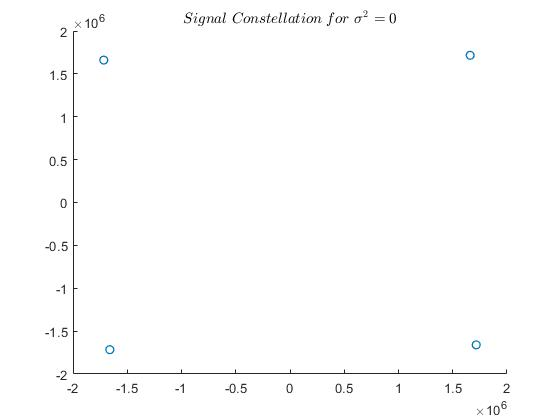
\includegraphics[width=0.9\textwidth]{untitled10.jpg}
\end{center}

\centering
نویز با واریانس ${\sigma}^2 = 0$
\\[1cm]


\begin{center}
    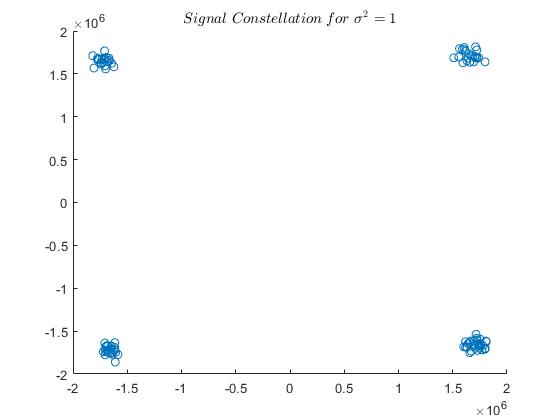
\includegraphics[width=0.9\textwidth]{untitled11.jpg}
\end{center}

\centering
نویز با واریانس ${\sigma}^2 = 1$
\\[0.5cm]


\begin{center}
    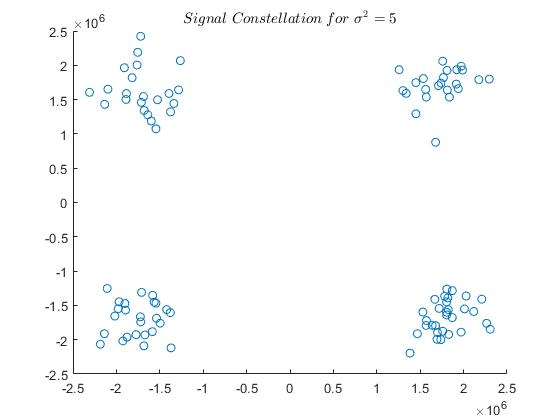
\includegraphics[width=0.9\textwidth]{untitled12.jpg}
\end{center}

\centering
نویز با واریانس ${\sigma}^2 = 5$
\\[1cm]


\begin{center}
    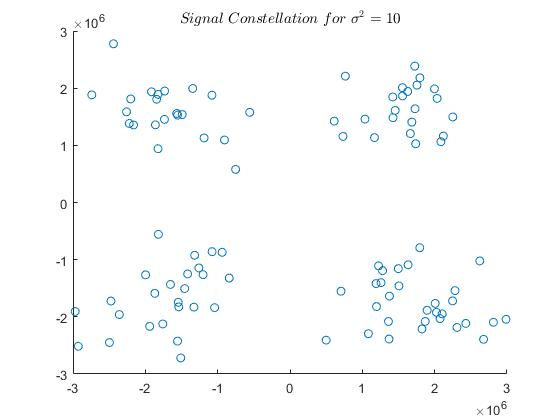
\includegraphics[width=0.9\textwidth]{untitled13.jpg}
\end{center}

\centering
نویز با واریانس ${\sigma}^2 = 10$
\\[0.5cm]


\begin{center}
    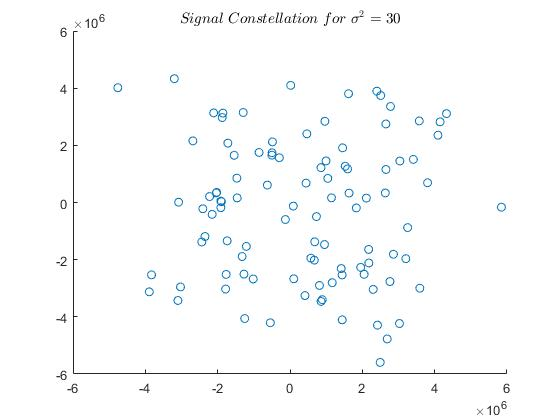
\includegraphics[width=0.9\textwidth]{untitled14.jpg}
\end{center}

\centering
نویز با واریانس ${\sigma}^2 = 30$
\\[1cm]


\begin{center}
    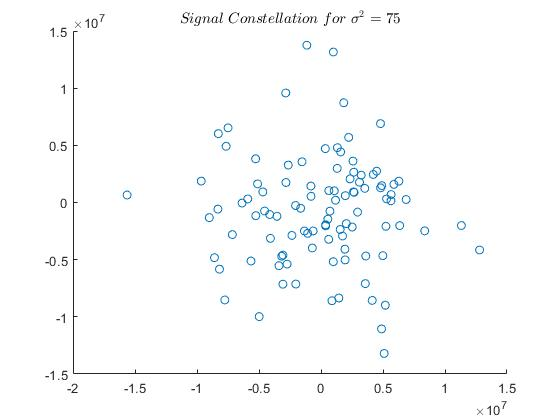
\includegraphics[width=0.9\textwidth]{untitled15.jpg}
\end{center}

\centering
نویز با واریانس ${\sigma}^2 = 75$
\\[0.5cm]

\justify
واضح است مطابق انتظار، هرچه نویز کمتر باشد تراکم این اعداد بازیابی شده باید بیشتر باشد. تا جایی که به ازای ${\sigma}^2 = 0$ نویز کاملا بر هم منطبق هستند. رفته رفته با افزایش واریانس نویز این نقاط از هم فاصله میگیرند تا جایی که به نظر میرسد برای واریانس های بسیار بالا اصلا هیچ تراکمی در منطقه خاصی وجود ندارد.
\\[1.5cm]
\large
3.2: 
کلیت این بخش و بخش قبل شباهت بسیار زیادی دارد. لذا از توضیحات تکراری پرهیز میکنیم و نتایج را به نمایش میگذاریم.
\\[1cm]
آ:
\\
خروجی های بلوک را به ترتیب نمایش میدهیم. شکل ها دارای Title، Xlabel و Ylabel میباشند.

\begin{center}
    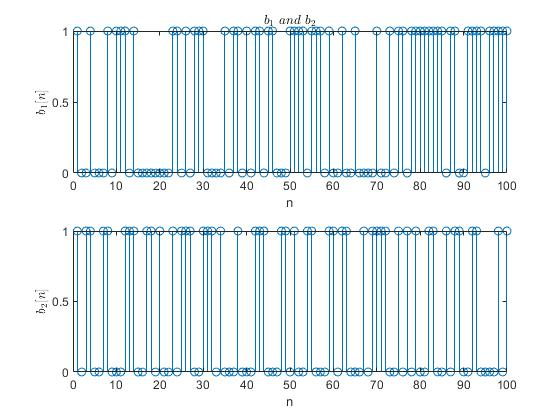
\includegraphics[width=0.9\textwidth]{untitled16.jpg}
\end{center}

\centering
خروجی تابع Divide


\begin{center}
    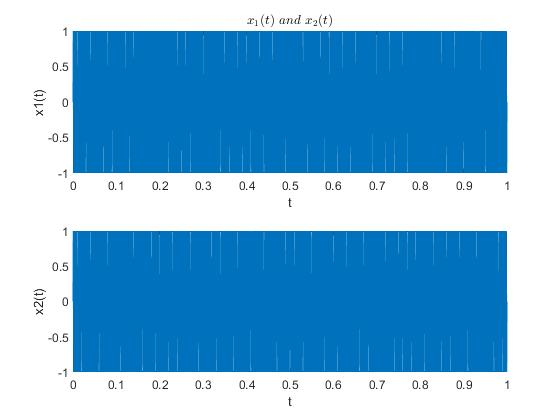
\includegraphics[width=0.9\textwidth]{untitled17.jpg}
\end{center}

\centering
خروجی تابع PulseShaping


\begin{center}
    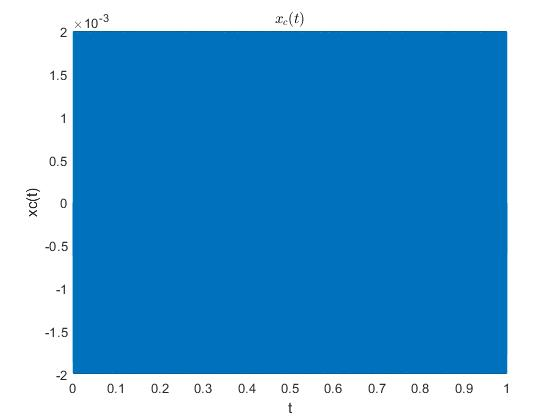
\includegraphics[width=0.9\textwidth]{untitled18.jpg}
\end{center}

\centering
خروجی تابع AnalogMod
 

\begin{center}
    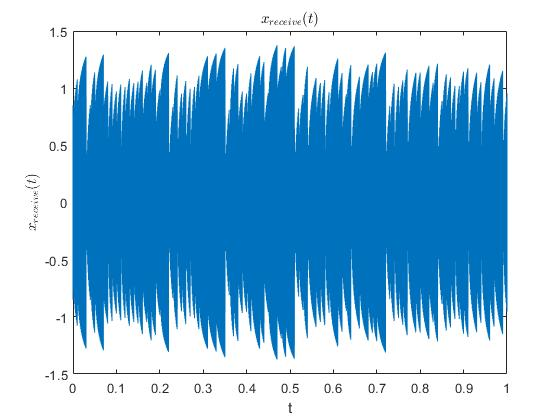
\includegraphics[width=0.9\textwidth]{untitled19.jpg}
\end{center}

\centering
خروجی تابع Channel
 

\begin{center}
    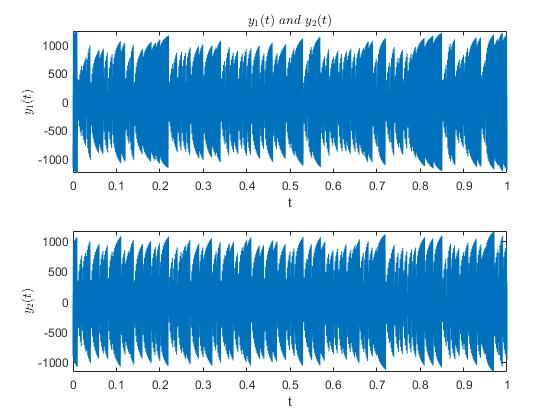
\includegraphics[width=0.9\textwidth]{untitled20.jpg}
\end{center}

\centering
خروجی تابع AnalogDemod
 

\begin{center}
    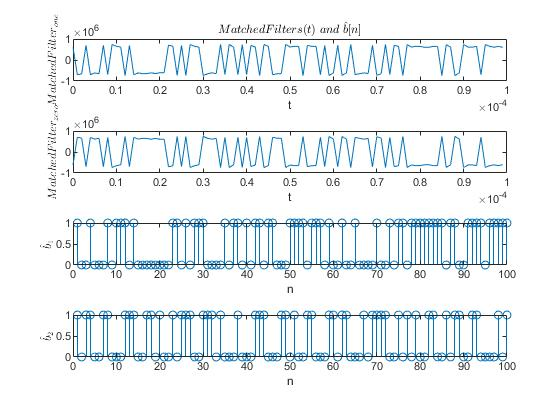
\includegraphics[width=0.9\textwidth]{untitled21.jpg}
\end{center}

\centering
خروجی تابع MatchedFilter
 

\begin{center}
    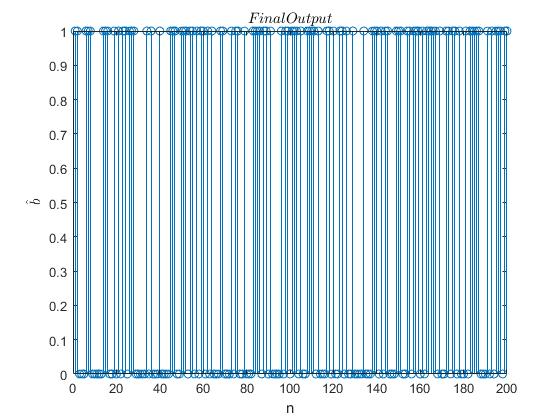
\includegraphics[width=0.9\textwidth]{untitled22.jpg}
\end{center}

\centering
خروجی تابع Combine
 

\begin{center}
    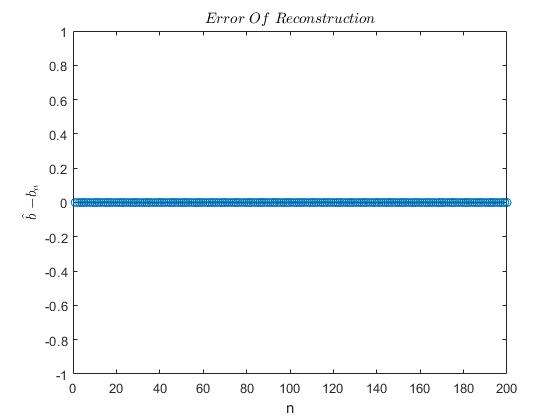
\includegraphics[width=0.9\textwidth]{untitled23.jpg}
\end{center}

\centering
خطای بازسازی


\raggedleft
ب:
\\
با استفاده از دستور normrnd در متلب که متغیر رندوم با توزیع گوسی و میانگین و واریانس دلخواه ما تولید میکند، به سیگنال خروجی از تابع Channel نویز می افزاییم. نتیجه خواسته شده به شرح زیر میباشد:


\begin{center}
    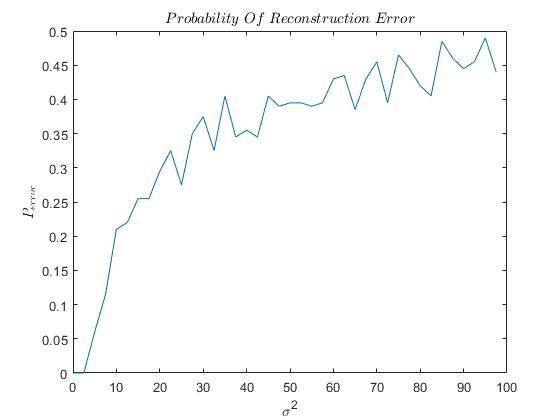
\includegraphics[width=0.9\textwidth]{untitled24.jpg}
\end{center}

\centering
احتمال خطای بازسازی برحسب واریانس نویز کانال
\\[0.5cm]
\raggedleft
\justify
واضح است انتظار داشتیم نتیجه ای مشابه با قسمت قبل را شاهد باشیم.البته تفاوت های ریزی نیز وجود دارد که در شکل واضح است. اما نکته مهم این است که همچنان مجموعهپ ما میتواند تا حدی اثر نویز را خنثی کند و بدون هیچ اشتباهی سیگنال را بازیابی کند. اما رفته رفته احتمال خطا بیشتر میشود تا اینکه اصلا به نزدیکی خطای 50 درصد میرسیم که یعنی اصلا یک سیگنال رندوم جدید تولید شده است (مشابه با علتی که در قسمت قبل توضیح دادیم)
\\
لازم به ذکر است رفتار کمی غیرخطی شکل فوق به این خاطر است که نمودار با 40 نمونه ترسیم شده تا زمان زیادی برای پردازش صرف نشود.
\\[1cm]



ج:
\\
بدون تکرار توضیحات مشابه قبل، نتایج شبیه سازی را با هم میبینیم:

\begin{center}
    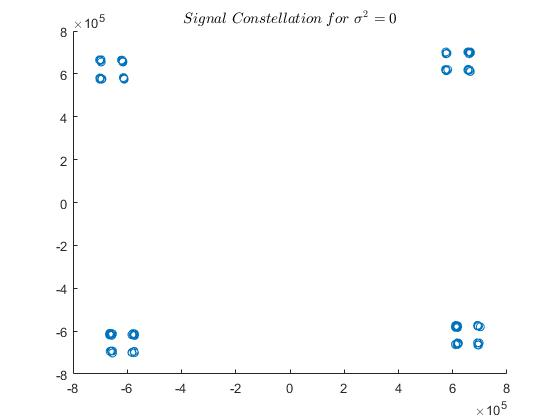
\includegraphics[width=0.9\textwidth]{untitled25.jpg}
\end{center}

\centering
نویز با واریانس ${\sigma}^2 = 0$
\\[1cm]


\begin{center}
    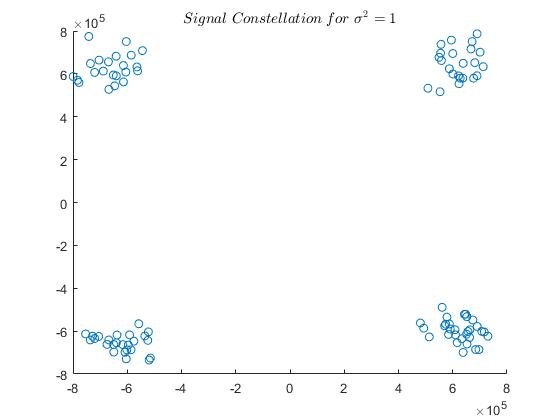
\includegraphics[width=0.9\textwidth]{untitled26.jpg}
\end{center}

\centering
نویز با واریانس ${\sigma}^2 = 1$
\\[0.5cm]


\begin{center}
    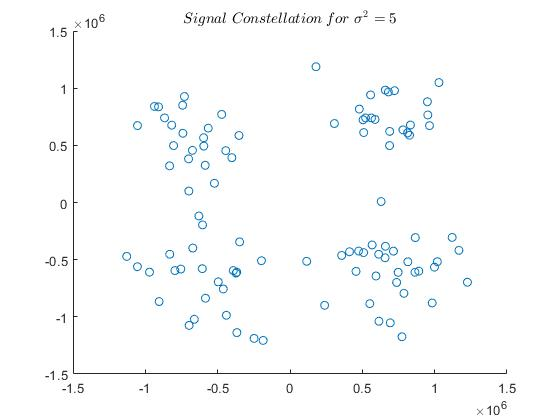
\includegraphics[width=0.9\textwidth]{untitled27.jpg}
\end{center}

\centering
نویز با واریانس ${\sigma}^2 = 5$
\\[1cm]


\begin{center}
    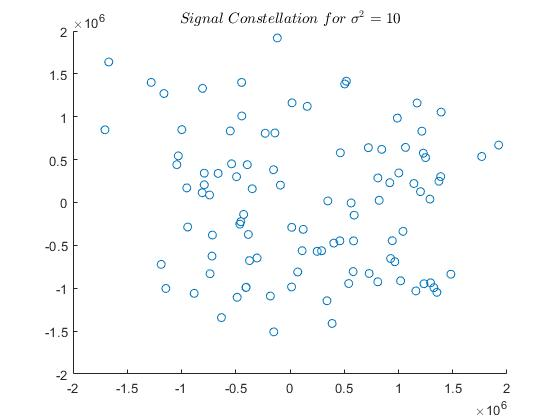
\includegraphics[width=0.9\textwidth]{untitled28.jpg}
\end{center}

\centering
نویز با واریانس ${\sigma}^2 = 10$
\\[0.5cm]


\begin{center}
    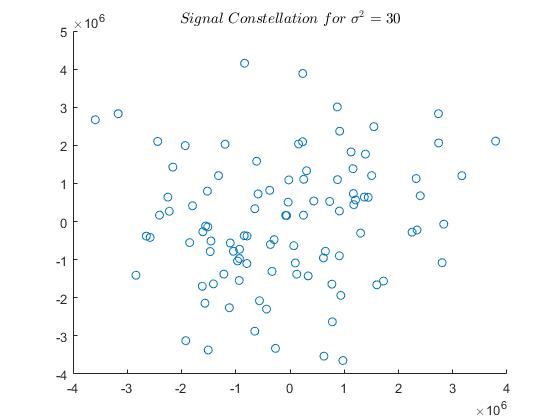
\includegraphics[width=0.9\textwidth]{untitled29.jpg}
\end{center}

\centering
نویز با واریانس ${\sigma}^2 = 30$
\\[1cm]


\begin{center}
    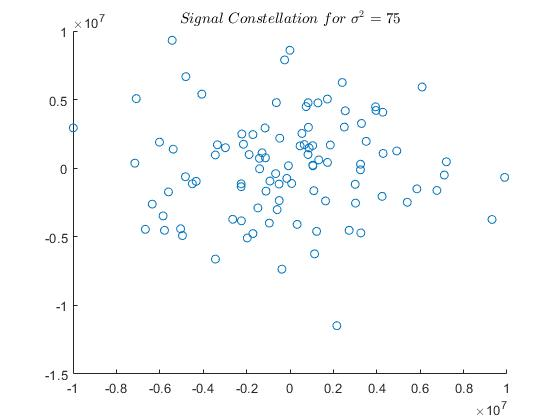
\includegraphics[width=0.9\textwidth]{untitled30.jpg}
\end{center}

\centering
نویز با واریانس ${\sigma}^2 = 75$
\\[0.5cm]

\justify
دو نکته مهم قابل بیان است. یکی اینکه با مقایسه با نتیجه این قسمت که در حالت PSK انجام شده با نتیجه قسمت قبل که حالت FSK بود، واضح است این روش نسبت به نویز کمی حساس تر است و زودتر منظومه سیگنال ها تراکم خودشان را از دست میدهند.
\\
نکته دوم نیز منظومه سیگنال ترسیم شده برای حالت ${\sigma^2}_{noise} = 0$ است که علی رغم اینکه تمام نقاط روی هم ترسیم نشده اند، اما همچنان از شکل میتوان استنباط کرد که فرایند بازسازی بدون خطا بوده است. علت اینکه در هر ناحیه بجای تمرکز بر یک نقطه، تمرکز بر چهار قسمت است این است که سیگنال های متناظر با بیت های ما سینوسی هستند. از طرفی فیلتر های ما با توجه به سبکی که تعریفشان کرده ایم ایده آل نیستند و برای همین در ابتدای سیگنال کمی دامنه آن ها کمتر است. به نوعی میتوان گفت سیگنال های خروجی از فیلتر ها یک بخش transient دارند و یک بخش state steady  که بخش گذرا باعث بوجود آمدن این پدیده شده است.


\large
3.3: 
کلیت این بخش و بخش قبل شباهت بسیار زیادی دارد. لذا از توضیحات تکراری پرهیز میکنیم و نتایج را به نمایش میگذاریم.
\\[1cm]

آ:
\\
بله، دو سیگنال متعامدند
باید ثابت کنیم که انتگرال حاصلضرب دو سیگنال روی یک دوره تناوب حاصلی برابر با صفر دارد:
\\
\[\int_{0}^{{T}_{s}} sin(2\pi\times1500\times t)sin(2\pi\times 1000\times t) \,dt = \frac{1}{2} \int_{0}^{{T}_{s}} {[}cos(2\pi\times500\times t)-cos(2\pi \times2500\times  t){]} \,dt  \]
\\
\[
=\frac{1}{2} {T}_{s} \frac{sin(2\pi\times 500\times {T}_{s})}{2\pi\times 500\times {T}_{s}} - \frac{1}{2} {T}_{s} \frac{sin(2\pi\times 2500\times {T}_{s})}{2\pi\times 2500\times {T}_{s}} \]
\\
و از آنجا که ${T}_{s} = integer$ بنابراین هر دو سینوس برابر صفر خواهند بود. لذا:
\\
\[\int_{0}^{{T}_{s}} sin(2\pi\times1500\times t)sin(2\pi\times 1000\times t) \,dt = 0\]
\\
اثبات شد.
\\[0.5cm]

ب:
\\
خروجی های بلوک را به ترتیب نمایش میدهیم. شکل ها دارای Title، Xlabel و Ylabel میباشند.

\begin{center}
    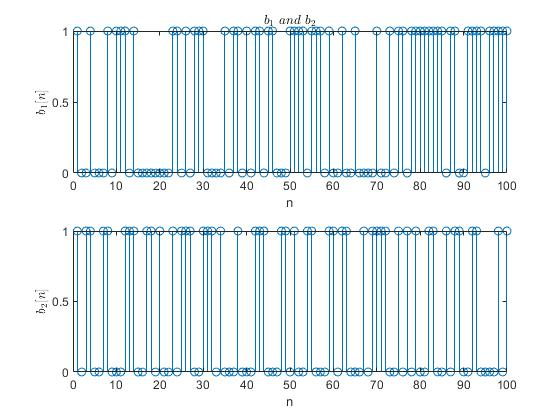
\includegraphics[width=0.9\textwidth]{untitled31.jpg}
\end{center}

\centering
خروجی تابع Divide


\begin{center}
    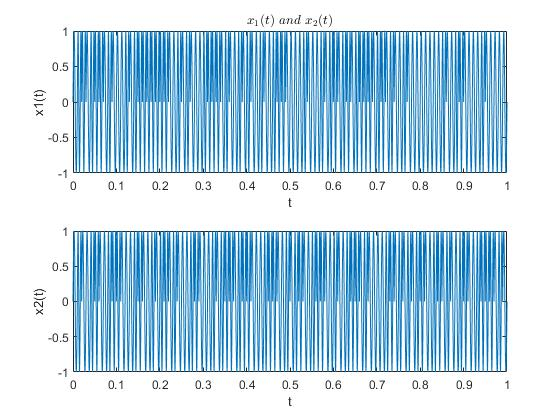
\includegraphics[width=0.9\textwidth]{untitled32.jpg}
\end{center}

\centering
خروجی تابع PulseShaping


\begin{center}
    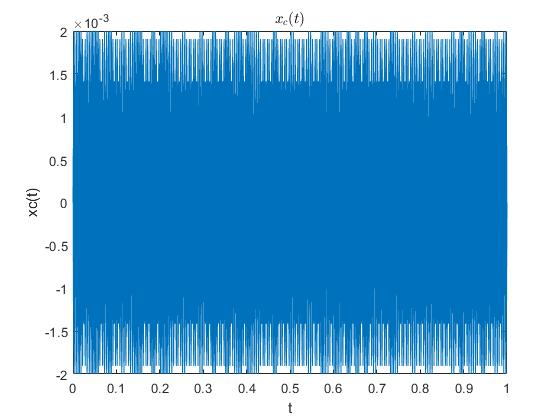
\includegraphics[width=0.9\textwidth]{untitled33.jpg}
\end{center}

\centering
خروجی تابع AnalogMod
 

\begin{center}
    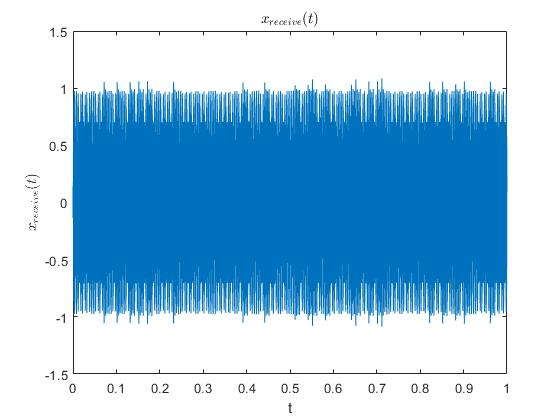
\includegraphics[width=0.9\textwidth]{untitled34.jpg}
\end{center}

\centering
خروجی تابع Channel
 

\begin{center}
    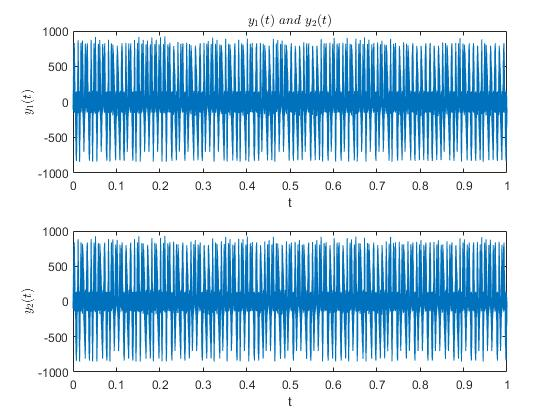
\includegraphics[width=0.9\textwidth]{untitled35.jpg}
\end{center}

\centering
خروجی تابع AnalogDemod
 

\begin{center}
    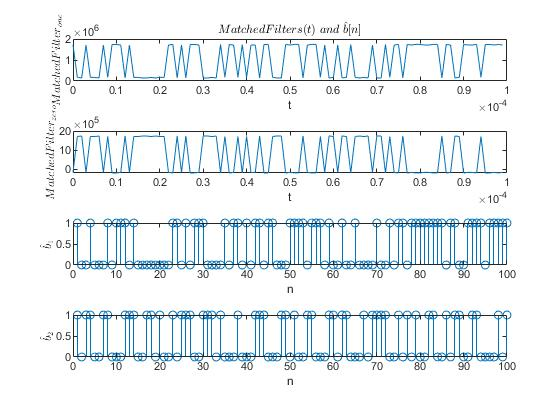
\includegraphics[width=0.9\textwidth]{untitled36.jpg}
\end{center}

\centering
خروجی تابع MatchedFilter
 

\begin{center}
    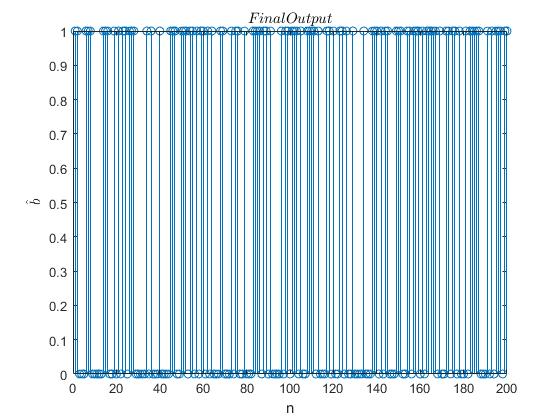
\includegraphics[width=0.9\textwidth]{untitled37.jpg}
\end{center}

\centering
خروجی تابع Combine
 

\begin{center}
    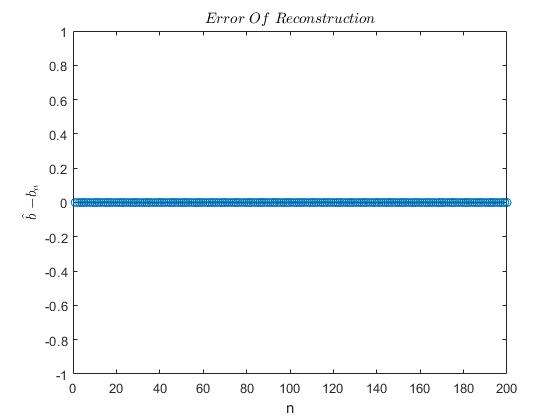
\includegraphics[width=0.9\textwidth]{untitled38.jpg}
\end{center}

\centering
خطای بازسازی


\raggedleft
ج:
\\
با استفاده از دستور normrnd در متلب که متغیر رندوم با توزیع گوسی و میانگین و واریانس دلخواه ما تولید میکند، به سیگنال خروجی از تابع Channel نویز می افزاییم. نتیجه خواسته شده به شرح زیر میباشد:


\begin{center}
    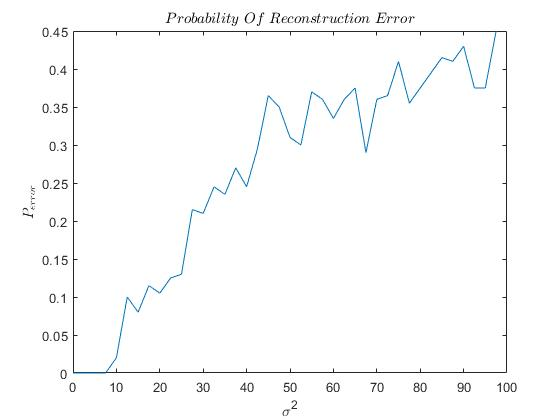
\includegraphics[width=0.9\textwidth]{untitled39.jpg}
\end{center}

\centering
احتمال خطای بازسازی برحسب واریانس نویز کانال
\\[0.5cm]
\raggedleft
\justify
واضح است انتظار داشتیم نتیجه ای مشابه با قسمت قبل را شاهد باشیم.البته تفاوت های ریزی نیز وجود دارد که در شکل واضح است. اما نکته مهم این است که همچنان مجموعه پروژه ما میتواند تا حدی اثر نویز را خنثی کند و بدون هیچ اشتباهی سیگنال را بازیابی کند. اما رفته رفته احتمال خطا بیشتر میشود تا اینکه اصلا به نزدیکی خطای 50 درصد میرسیم که یعنی اصلا یک سیگنال رندوم جدید تولید شده است (مشابه با علتی که در قسمت قبل توضیح دادیم)
\\
لازم به ذکر است رفتار کمی غیرخطی شکل فوق به این خاطر است که نمودار با 40 نمونه ترسیم شده تا زمان زیادی برای پردازش صرف نشود.
\\[1cm]



د:
\\
بدون تکرار توضیحات مشابه قبل، نتایج شبیه سازی را با هم میبینیم:

\begin{center}
    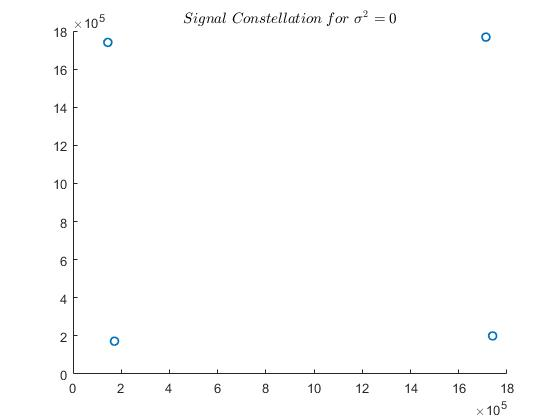
\includegraphics[width=0.9\textwidth]{untitled40.jpg}
\end{center}

\centering
نویز با واریانس ${\sigma}^2 = 0$
\\[1cm]


\begin{center}
    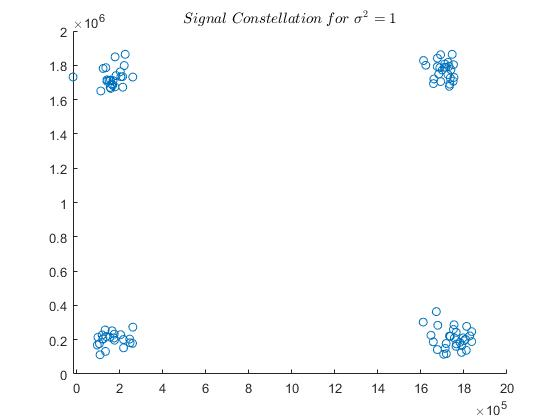
\includegraphics[width=0.9\textwidth]{untitled41.jpg}
\end{center}

\centering
نویز با واریانس ${\sigma}^2 = 1$
\\[0.5cm]


\begin{center}
    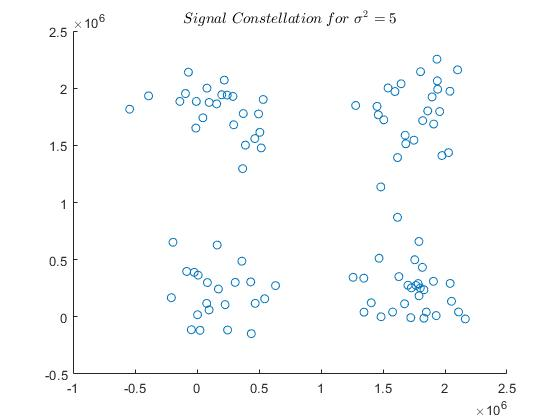
\includegraphics[width=0.9\textwidth]{untitled42.jpg}
\end{center}

\centering
نویز با واریانس ${\sigma}^2 = 5$
\\[1cm]


\begin{center}
    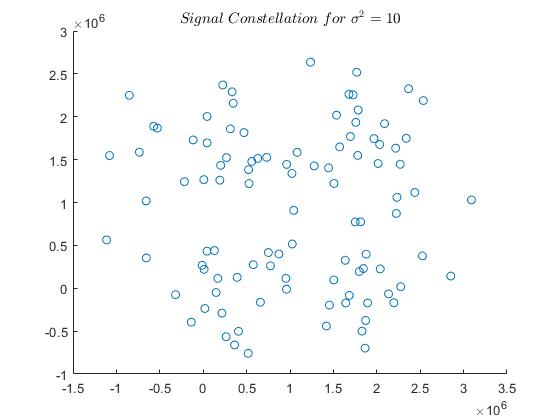
\includegraphics[width=0.9\textwidth]{untitled43.jpg}
\end{center}

\centering
نویز با واریانس ${\sigma}^2 = 10$
\\[0.5cm]


\begin{center}
    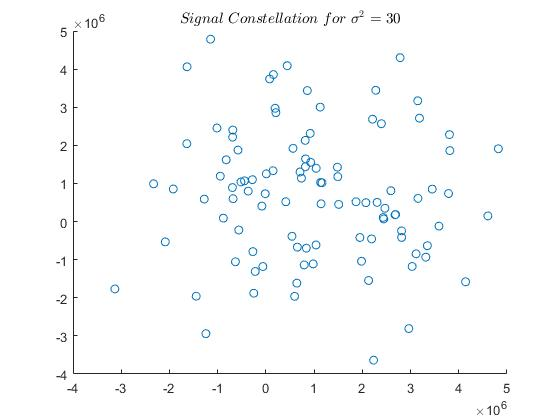
\includegraphics[width=0.9\textwidth]{untitled44.jpg}
\end{center}

\centering
نویز با واریانس ${\sigma}^2 = 30$
\\[1cm]


\begin{center}
    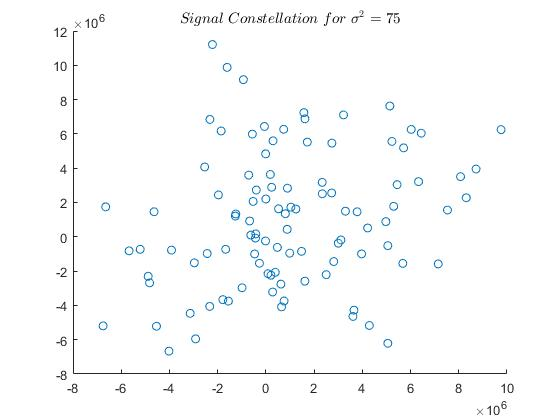
\includegraphics[width=0.9\textwidth]{untitled45.jpg}
\end{center}

\centering
نویز با واریانس ${\sigma}^2 = 75$
\\[0.5cm]

\justify
میبینیم که مدولاسیون FSK از خود مقاومت خوبی نشان داده و منظومه های سیگنال شکل های خوب و متراکمی هستند. البته که بدیهتا در این حالت نیز به ازای واریانس نویز بزرگ، منظومه از تراکم خارج شده و در کل صفحه پخش میشود.
\\[1.5cm]

\newpage
\huge
\section{انتقال دنباله ای از اعداد 8 بیتی}
\large
در این بخش ابتدا سیگنال هایی با اندازه های بین مقادیر 0 تا 255 را جداگانه به باینری تبدیل میکنیم و سپس آن هارا از طریق سازوکاری که تولید کرده ایم مدوله میکنیم. مجددا بیت های باینری مدوله شده را به اعداد دسیمال تبدیل میکنیم و انتظار داریم اعدادی که تولید کرده ایم با چیزی که ارسال کرده ایم مشابه باشند.
\\[1cm]

4.1:
تابع SourceGenerator را مطابق عملکردی که باید طراحی کرده ایم. لازم به ذکر است که تابع de2bi استفاده شده در این قسمت، یک ماتریس خروجی میدهد که ما سطر های مختلف این ماتریس را در کنار هم قرار داده ایم تا خروجی دلخواه تولید شود.
\\
برای تابع SourceDecoder نیز روند مشابهی طی کردیم و از تابع bi2de استفاده کرده و 8 بیت 8 بیت را با استفاده از این تابع به اعداد دسیمال تبدیل کرده ایم.
\\[0.5cm]
\large
4.2:
طبق تعریف سوال، خطای بازسازی برابر با مجذور اختلاف اعداد است. با این تعریف نتیجه این بخش مشابه زیر میباشد:

\begin{center}
    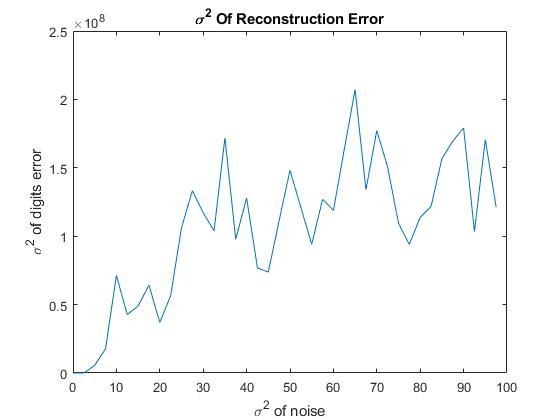
\includegraphics[width=0.9\textwidth]{untitled46.jpg}
\end{center}

\centering
واریانس خطا برحسب واریانس نویز
\\[1cm]
\justify
واضح است که زمانی که واریانس نویز کم است، بازسازی اعداد دسیمال بدون خطا بوده و بنابراین واریانس خطا نیز صفر است. رفته رفته با افزایش واریانس نویز، تعداد و مقدار خطای بازسازی اعداد دسیمال بیشتر شده به نحوی که به ازای نویز های بسیار بزرگ، اعداد دسیمال های بازسازی شده را میتوان اعداد رندوم بین 0 تا 255 فرض کرد. برای همین واریانس خطا نیز یک متغیر تصادفی جدید است که میتواند مقادیر بسیار بزرگی اتخاذ کند که در تصویر نیز واضح است.
\\[0.5cm]
\large
4.3:
خواسته مساله را به ازای واریانس های مختلف ترسیم میکنیم که نتیجه به شرح زیر است:

\begin{center}
    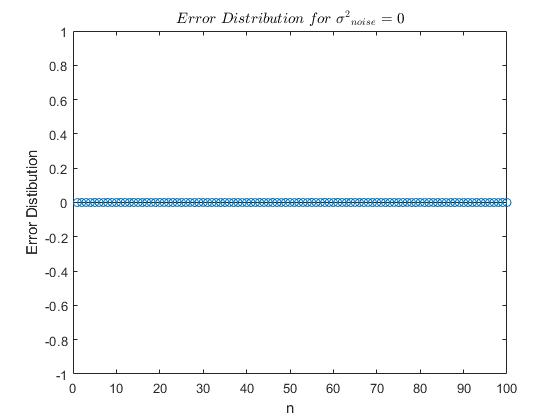
\includegraphics[width=0.9\textwidth]{untitled47.jpg}
\end{center}

\centering
تابع توزیع خطا برای ${\sigma^2}_{noise} = 0$
\\[1cm]


\begin{center}
    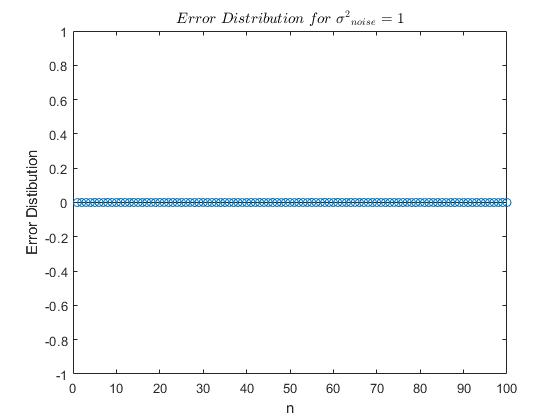
\includegraphics[width=0.9\textwidth]{untitled48.jpg}
\end{center}

\centering
تابع توزیع خطا برای ${\sigma^2}_{noise} = 1$
\\[1cm]


\begin{center}
    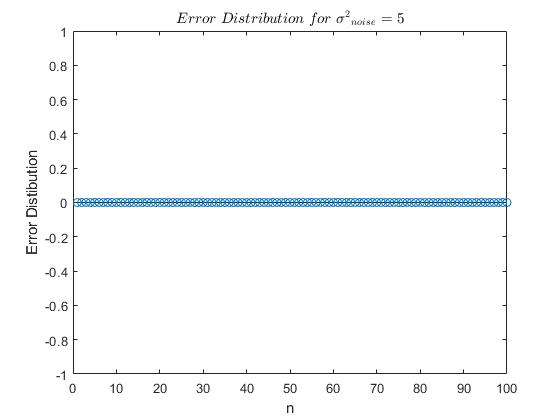
\includegraphics[width=0.9\textwidth]{untitled49.jpg}
\end{center}

\centering
تابع توزیع خطا برای ${\sigma^2}_{noise} = 5$
\\[1cm]


\begin{center}
    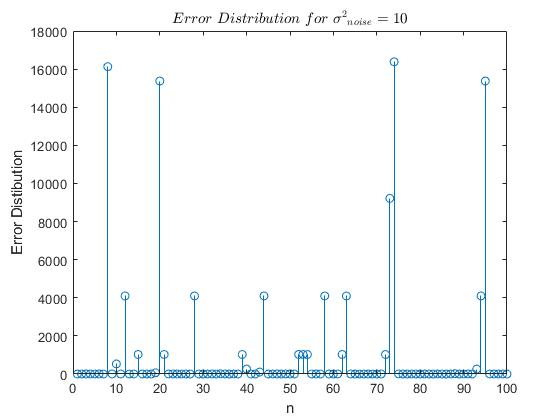
\includegraphics[width=0.9\textwidth]{untitled50.jpg}
\end{center}

\centering
تابع توزیع خطا برای ${\sigma^2}_{noise} = 10$
\\[1cm]


\begin{center}
    \includegraphics[width=0.9\textwidth]{untitled51.jpg}
\end{center}

\centering
تابع توزیع خطا برای ${\sigma^2}_{noise} = 25$
\\[1cm]


\begin{center}
    \includegraphics[width=0.9\textwidth]{untitled52.jpg}
\end{center}

\centering
تابع توزیع خطا برای ${\sigma^2}_{noise} = 70$
\\[1cm]


\begin{center}
    \includegraphics[width=0.9\textwidth]{untitled53.jpg}
\end{center}

\centering
تابع توزیع خطا برای ${\sigma^2}_{noise} = 150$
\\[1cm]


\begin{center}
    \includegraphics[width=0.9\textwidth]{untitled54.jpg}
\end{center}

\centering
تابع توزیع خطا برای ${\sigma^2}_{noise} = 500$
\\[1cm]

\justify
مطابق انتظار، توزیع خطا برای واریانس های کم توزیع ثابت صفر است. چرا که بازسازی اعداد دسیمال بدون هیچ خطایی انجام میشود. اما با افزایش نویز خطا کم کم در باز سازی ظاهر میشود تا جایی که برای نویز های بزرگ، عملا توزیع خطا را میتوان حاصل تفریق دو عدد رندوم میان 0 تا 250 دانست  برای همین خود تابع توزیع برای واریانس های بزرگ نیز میتواند تمام مقادیر این بازه را  (البته مجذور آن را) اختیار کند.
پس انتظار داریم هر عددی در بازه ${0}^2$ الی ${255}^2$ را ملاحظه کنیم که همینطور نیز هست.
\\[0.5cm]
4.4:
\\
توزیع خطا را هنگامی که نویز به بینهایت میل میکند میابیم. لازم به ذکر است که گفتیم که زمانی که نویز به بینهایت میل میکند سیگنال بازسازی شده کاملا یک سیگنال رندوم جدید است و کلید حل این مسئله، در مستقل بودن سیگنال بازسازی شده از سیگنال ارسالی است. خواهیم داشت:
\\
\[
X_n(x) \sim Uinform(0,255)\  {  and  }\ {Y_n}(x) \sim Uniform(0,255)\ {  and  }\ {  independent  } \rightarrow  
\]
\\
\[
Z=X-Y \sim \Lambda(-255,255)
\]
\\
پس با توجه به توزیع خطا، واضح است که واریانس با رفتاری که از شبیه سازی دیدیم متشابه است.






\newpage
\huge
\section{کدینگ منبع}
\large
5.1:
با فرض منبع داده شده و کدینگ های مفروض:
\\[0.5cm]
آ:
\\
واضح است کد مربوط به دو حرف b و d یکسان و برابر 10 میباشد. بنابراین گیرنده با مشاهده کد 10 نمیتواند تشخیص دهد کدام یک از حروف b یا d ارسال شده بوده است
\\[0.3cm]
ب:
\\
کدگذاری سمبل ها نباید به نحوی باشد که کنارهم قرار گرفتن آن ها باعث تولید یک کد دیگر از همان مجموعه شود. یعنی فرض کنید که فرستنده 'ab' را ارسال میکند که به 010 کد میشود. همینطور اگر 'd' را کد کرده و ارسال کند لازم است 010 ارسال شود. حال گیرنده چگونه میتواند تشخیص دهد تفاوت میان این دو کدینگ یکسان 010 چیست و در نتیجه این دیکود را نمیتوان تشخیص داد
\\[0.3cm]
ج:
\\
همانطور که مساله نیز توضیح داده است، با این نوع کدینگ نمیتوان تصمیم آنی گرفت. یعنی مثلا فرض کنید در گیرنده بیت 0 دیده میشود. حال میتواند تصمیم بگیرد که این 0 را به حرف a دیکود کند و میتواند صبر کند تا بیت بعدی را دریافت کند. حال فرض کنید بیت بعدی 1 بود. مجددا میتواند این مجموعه 01 را به حرف b دیکود کند یا میتواند منتظر بماند تا بیت بعدی دریافت شود و همین مشکل تا آخر ادامه میابد.
\\[0.5cm]
5.2:
\\
با توجه به راهنمایی خود مساله، موقتا مساله لاگرانژ را برای حالت تساوی حل میکنیم و از نتیجه آن استنباط لازم را انجام میدهیم:
\\[0.3cm]
دو معادله زیر را تشکیل میدهیم:
\\
\[{1: } \sum_{i=1}^{M} 2^{-l_{i}} = \frac{1}{2^{l_{a}}} + \frac{1}{2^{l_{b}}} + \frac{1}{2^{l_{c}}} + \frac{1}{2^{l_{d}}} + \frac{1}{2^{l_{e}}} + \frac{1}{2^{l_{f}}} = 1  \]
\\
\[
 \nabla F(l_a,l_b,l_c,l_d,l_e,l_f) =
\nabla \sum_{i=1}^{M} {p}_{i}{l}_i = \lambda \nabla \sum_{i=1}^{M} 2^{-l_{i}} =
\lambda \nabla G(l_a,l_b,l_c,l_d,l_e,l_f)
\rightarrow 
\]
\\
\[
{2:} <F_{l_a}, F_{l_b}, F_{l_c}, F_{l_d}, F_{l_e}, F_{l_f}> = <\lambda G_{l_a},\lambda G_{l_b},\lambda G_{l_c},\lambda G_{l_d},\lambda G_{l_e},\lambda G_{l_f}>
\]
\\
\raggedleft
\\
از حل دو معادله فوق نتیجه زیر حاصل میشود:
\\[0.3cm]
\centering
$l_a=1, l_b=2, l_c=3, l_d=4, l_e=5, l_f=5$
\\[0.5cm]
\raggedleft
5.3:
\\
با توجه به حالاتی که در قسمت قبل توضیح داده شده و نتیجه ای که خودمان پیدا کردیم، یک کدگذاری ممکن به صورت زیر خواهد بود:
\\[0.3cm]
\centering
$a=0, b=10, c=110, d=1110, e=11110, f=11111$
\\[0.5cm]
\raggedleft
5.4:
\\
طول متوسط کد ها برابر است با:
\\[0.3cm]
\[
\bar{l} = \frac{1+2+3+4+5+5}{6} = 3.33
\]
\\[0.5cm]
5.5 الی 5.7:
\\
توابع خواسته شده در این بخش هارا تولید کردیم. نکته خاصی در تولید این توابع وجود نداشت و توضیحات لازمه را در صورت نیاز در کد کامنت کرده ایم.
احتمالات موجود در قسمت اول سوال که بیان شد(حروف) را با اعداد در اینجا هم ارز کرده ایم و احتمالات هر کدام را با توجه به آن نوشته و به طور کامل توابع در کد نشان داده شده اند
\\[0.5cm]
5.8:
\\
برای قطعه کد این بخش نیز در هر مرحله تصویر را بررسی کنیم و اگر دو حالت برابر بودند counterرا یک واحذ اضافه میکنیم و اگر در for ما counterبرابر 10شود این یعنی نتیجه درستی گرفته ایم و true پرینت می شود
\\

\begin{center}
    \includegraphics[width=0.9\textwidth]{untitled56.jpg}
\end{center}


5.9:
\\
\begin{center}
    \includegraphics[width=0.9\textwidth]{untitled55.jpg}
\end{center}

\centering

$H_n(X) = \frac{L_avg}{n} $ بر حسب n
\\
واضح است که برای مقادیر n کوچک مقدار مورد بررسی عدد مشخصی ندارد. اما با افزایش تعداد سیمبول ها، مقدار میانگین طول به عددی نزدیک 2 میل میکند. حالا نتیجه ریاضی را بررسی میکنیم:
\\
\[
l_0=1,p_0=\frac{1}{2};l_(250)=2,p_(250)=\frac{1}{4};l_(100)=3,p_(100)=\frac{1}{8};l_(150)=4,p_(150)=\frac{1}{16}
\]
\[
l_(200)=5,p_(200)=\frac{1}{32};l_(50)=5,p_(50)=\frac{1}{32}
\]
\\
\[
\bar{length}=\frac{1}{2}\times 1 + \frac{1}{4}\times 2 + \frac{1}{8}\times 3 + \frac{1}{16}\times 4 + \frac{1}{32}\times 3  + \frac{1}{32}\times 5 = 1.9375
\]
\raggedleft
\\
پس در حالت تئوریک انتظار داریم به عدد 9375.1 میل کنیم که در تصویر حاصل از شبیه سازی نیز این کاملا مشهود است.
